\documentclass{article}
\usepackage{listings}
\usepackage{graphicx}
\usepackage{color}

\definecolor{mygreen}{rgb}{0,0.6,0}
\definecolor{mygray}{rgb}{0.5,0.5,0.5}
\definecolor{mymauve}{rgb}{0.58,0,0.82}

\lstset{ %
  backgroundcolor=\color{white},   % choose the background color; you must add \usepackage{color} or \usepackage{xcolor}; should come as last argument
  basicstyle=\footnotesize,        % the size of the fonts that are used for the code
  breakatwhitespace=false,         % sets if automatic breaks should only happen at whitespace
  breaklines=true,                 % sets automatic line breaking
  captionpos=b,                    % sets the caption-position to bottom
  commentstyle=\color{mygreen},    % comment style
  deletekeywords={...},            % if you want to delete keywords from the given language
  escapeinside={\%*}{*)},          % if you want to add LaTeX within your code
  extendedchars=true,              % lets you use non-ASCII characters; for 8-bits encodings only, does not work with UTF-8
  frame=single,	                   % adds a frame around the code
  keepspaces=true,                 % keeps spaces in text, useful for keeping indentation of code (possibly needs columns=flexible)
  keywordstyle=\color{blue},       % keyword style
  language=Octave,                 % the language of the code
  morekeywords={*,...},           % if you want to add more keywords to the set
  numbers=left,                    % where to put the line-numbers; possible values are (none, left, right)
  numbersep=5pt,                   % how far the line-numbers are from the code
  numberstyle=\tiny\color{mygray}, % the style that is used for the line-numbers
  rulecolor=\color{black},         % if not set, the frame-color may be changed on line-breaks within not-black text (e.g. comments (green here))
  showspaces=false,                % show spaces everywhere adding particular underscores; it overrides 'showstringspaces'
  showstringspaces=false,          % underline spaces within strings only
  showtabs=false,                  % show tabs within strings adding particular underscores
  stepnumber=2,                    % the step between two line-numbers. If it's 1, each line will be numbered
  stringstyle=\color{mymauve},     % string literal style
  tabsize=2,	                   % sets default tabsize to 2 spaces
  title=\lstname                   % show the filename of files included with \lstinputlisting; also try caption instead of title
}

\author{Jacob Hutter, Junhao Pan}
\title{ECE 313 Final Project Report}

\begin{document}
\maketitle


\underline{\textbf{Task 0:}}
\begin{lstlisting}
    clear all;
    clc;

    load 1_a41178.mat;
    patient1_data = floor(all_data);
    patient1_labels = all_labels;
    training1 = patient1_data(:,1:(2*length(patient1_data)/3));
    testing1 = patient1_data(:,(2*length(patient1_data)/3):length(patient1_data));
    label_training1 = patient1_labels(1:(2*length(patient1_labels)/3));
    label_testing1 = patient1_labels((2*length(patient1_labels)/3):length(patient1_labels));

    load 2_a42126.mat;
    patient2_data = floor(all_data);
    patient2_labels = all_labels;
    training2 = patient2_data(:,1:floor(2*length(patient2_data)/3));
    testing2 = patient2_data(:,floor(2*length(patient2_data)/3):length(patient2_data));
    label_training2 = patient2_labels(1:floor(2*length(patient2_labels)/3));
    label_testing2 = patient2_labels(floor(2*length(patient2_labels)/3):length(patient2_labels));

    load 3_a40076.mat;
    patient3_data = floor(all_data);
    patient3_labels = all_labels;
    training3 = patient3_data(:,1:(2*length(patient3_data)/3));
    testing3 = patient3_data(:,(2*length(patient3_data)/3):length(patient3_data));
    label_training3 = patient3_labels(1:(2*length(patient3_labels)/3));
    label_testing3 = patient3_labels((2*length(patient3_labels)/3):length(patient3_labels));

    load 4_a40050.mat;
    patient4_data = floor(all_data);
    patient4_labels = all_labels;
    training4 = patient4_data(:,1:floor(2*length(patient4_data)/3));
    testing4 = patient4_data(:,floor(2*length(patient4_data)/3):length(patient4_data));
    label_training4 = patient4_labels(1:floor(2*length(patient4_labels)/3));
    label_testing4 = patient4_labels(floor(2*length(patient4_labels)/3):length(patient4_labels));

    load 5_a41287.mat;
    patient5_data = floor(all_data);
    patient5_labels = all_labels;
    training5 = patient5_data(:,1:(2*length(patient5_data)/3));
    testing5 = patient5_data(:,(2*length(patient5_data)/3):length(patient5_data));
    label_training5 = patient5_labels(1:(2*length(patient5_labels)/3));
    label_testing5 = patient5_labels((2*length(patient5_labels)/3):length(patient5_labels));

    load 6_a41846.mat;
    patient6_data = floor(all_data);
    patient6_labels = all_labels;
    training6 = patient6_data(:,1:floor(2*length(patient6_data)/3));
    testing6 = patient6_data(:,floor(2*length(patient6_data)/3):length(patient6_data));
    label_training6 = patient6_labels(1:floor(2*length(patient6_labels)/3));
    label_testing6 = patient6_labels(floor(2*length(patient6_labels)/3):length(patient6_labels));

    load 7_a41846.mat;
    patient7_data = floor(all_data);
    patient7_labels = all_labels;
    training7 = patient7_data(:,1:floor(2*length(patient7_data)/3));
    testing7 = patient7_data(:,floor(2*length(patient7_data)/3):length(patient7_data));
    label_training7 = patient7_labels(1:floor(2*length(patient7_labels)/3));
    label_testing7 = patient7_labels(floor(2*length(patient7_labels)/3):length(patient7_labels));

    load 8_a42008.mat;
    patient8_data = floor(all_data);
    patient8_labels = all_labels;
    training8 = patient8_data(:,1:(2*length(patient8_data)/3));
    testing8 = patient8_data(:,(2*length(patient8_data)/3):length(patient8_data));
    label_training8 = patient8_labels(1:(2*length(patient8_labels)/3));
    label_testing8 = patient8_labels((2*length(patient8_labels)/3):length(patient8_labels));

    load 9_a41846.mat;
    patient9_data = floor(all_data);
    patient9_labels = all_labels;
    training9 = patient9_data(:,1:floor(2*length(patient9_data)/3));
    testing9 = patient9_data(:,floor(2*length(patient9_data)/3):length(patient9_data));
    label_training9 = patient9_labels(1:floor(2*length(patient9_labels)/3));
    label_testing9 = patient9_labels(floor(2*length(patient9_labels)/3):length(patient9_labels));
\end{lstlisting}
For task 0 we took the raw patient and gold data and partitioned it into testing and training segments.
\\ \underline{\textbf{Task 1.1:}}
\begin{lstlisting}
HT_table_array_pat_1 = Get_HT_table(1, training1, label_training1);
HT_table_array_pat_2 = Get_HT_table(2, training2, label_training2);
HT_table_array_pat_3 = Get_HT_table(3, training3, label_training3);
HT_table_array_pat_4 = Get_HT_table(4, training4, label_training4);
HT_table_array_pat_5 = Get_HT_table(5, training5, label_training5);
HT_table_array_pat_6 = Get_HT_table(6, training6, label_training6);
HT_table_array_pat_7 = Get_HT_table(7, training7, label_training7);
HT_table_array_pat_8 = Get_HT_table(8, training8, label_training8);
HT_table_array_pat_9 = Get_HT_table(9, training9, label_training9);

HT_table_array = cat(1, HT_table_array_pat_1, HT_table_array_pat_2, HT_table_array_pat_3, HT_table_array_pat_4, HT_table_array_pat_5, HT_table_array_pat_6, HT_table_array_pat_7, HT_table_array_pat_8, HT_table_array_pat_9);
\end{lstlisting}
\begin{lstlisting}
function HT_table_array_pat = Get_HT_table(patient_index, patient_data, patient_labels)

% Prior probablities, alarms/total
P_H1 = sum(patient_labels)/length(patient_labels);
P_H0 = 1 - P_H1;

HT_table_array_pat = cell(1, 7);

% name = strcat('Patient_', int2str(patient_index), '_Features');
% figure('name', name, 'unit', 'normalized', 'outerposition', [.1 .1 .8 .8]);

for i = 1:7
	[feature_mat, x_mat] = Get_Feat_Mat(patient_data(i:i, :), patient_labels);

	ML_vector = zeros(1, length(feature_mat(1:1, :)));
	MAP_vector = zeros(1, length(feature_mat(1:1, :)));

	for k = 1:length(feature_mat(1:1, :))
		P_H1_i = feature_mat(1, k);
		P_H0_i = feature_mat(2, k);
		if (P_H1_i >= P_H0_i)
			% if H1_pmf >= H0_pmf
			ML_vector(k) = 1;
		end
		if (P_H1*P_H1_i >= P_H0*P_H0_i)
			% if H1_pmf*P(H1) >= H0_pmf*P(H0)
			MAP_vector(k) = 1;
		end
	end

	HT_table = cat(1, x_mat, feature_mat(1:1, :), feature_mat(2:2, :), ML_vector, MAP_vector);
	HT_table = rot90(HT_table, -1);
	HT_table = fliplr(HT_table);
	% Have to flip the table so that it matches with the given format
	HT_table_array_pat{1, i} = num2cell(HT_table);
	subplot(7, 1, i);
 	hold on;
 	plot(x_mat, feature_mat(1:1, :));
 	plot(x_mat, feature_mat(2:2, :));
 	legend('H0 pmf', 'H1 pmf');
 	hold off;
end
\end{lstlisting}
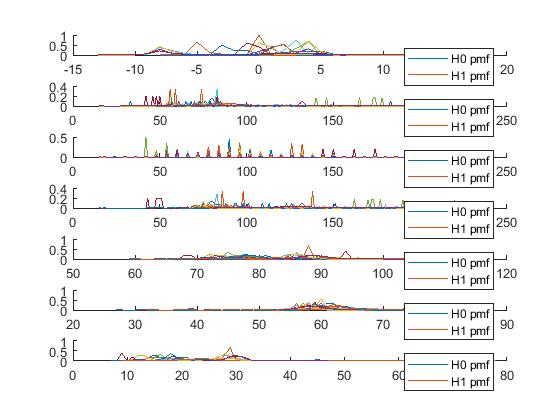
\includegraphics[scale = 1]{untitled}
\underline{\textbf{Task 1.2:}}
\end{document}
